\section{Physical problem and mathematical formulation}

\subsection{Computational Domain and Prescribed Velocity Field}

The computational domain is a two-dimensional rectangular channel with length $L_x=5$ and height $L_y=1$, as illustrated in Fig.~\ref{fig:computational_domain}. A prescribed unidirectional velocity field is considered, given by

\begin{equation}
    u(y)=18y(1-y),
    \qquad
    v(y)=0,
    \label{eq:velocity_field}
\end{equation}

where $u$ and $v$ denote the streamwise and wall-normal velocity components, respectively. The streamwise velocity follows a parabolic profile, with a maximum value of $u_{\max}=4.5$ at the channel centreline ($y=0.5$), and vanishes at both walls.

The mean streamwise velocity is obtained by integrating the velocity profile over the channel height:

\begin{equation}
    \bar{u}
    =\frac{1}{L_y}\int_0^{L_y}u(y)\,dy
    =\int_0^1 18y(1-y)\,dy
    =3.
\end{equation}

Thus, the prescribed velocity profile corresponds to a mean velocity of $3$. The velocity field is not obtained by solving the momentum equations; instead, it is specified analytically and held fixed throughout the parameter studies. Accordingly, only the temperature field is computed from the governing energy equation.

\begin{figure}[htbp]
    \centering
    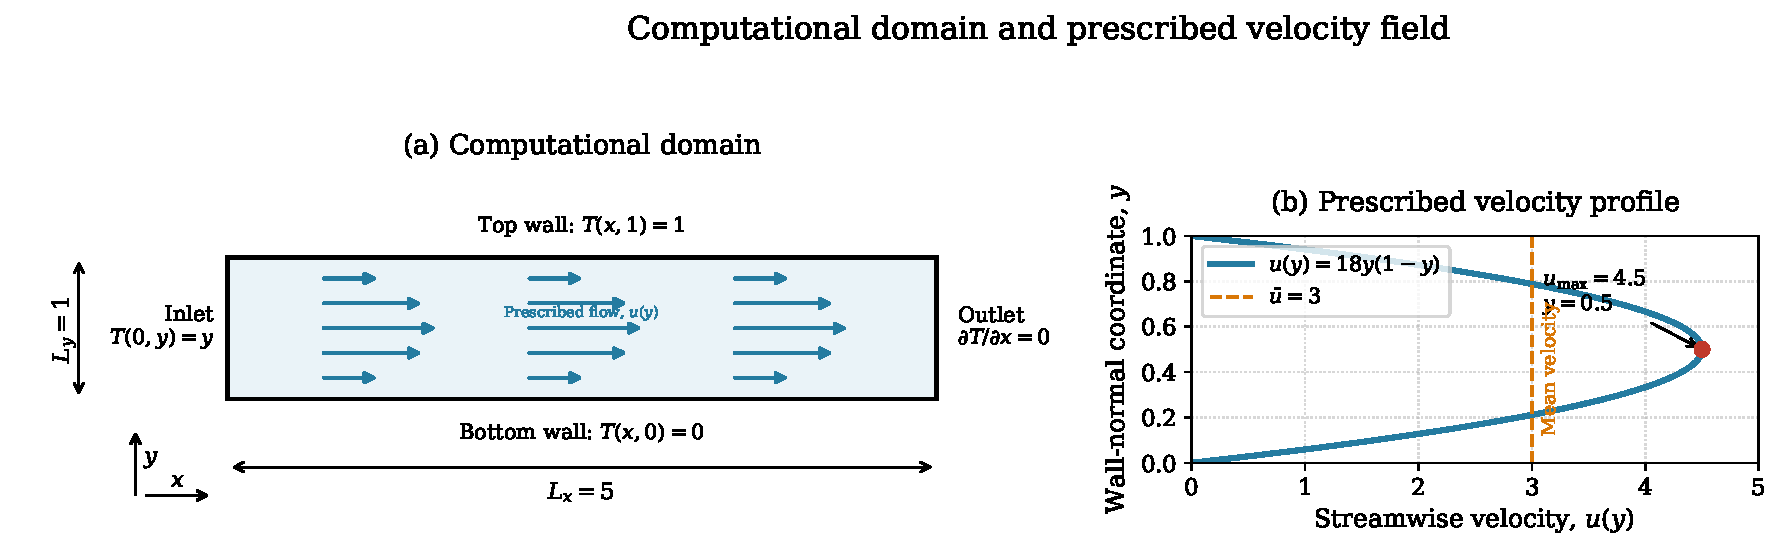
\includegraphics[width=0.90\textwidth]
    {figures/computational_domain_velocity_profile.pdf}
    \caption{Computational domain, thermal boundary conditions, and prescribed parabolic velocity profile.}
    \label{fig:computational_domain}
\end{figure}

\subsection{Governing Energy Equation}

The energy equation describes the temperature field under the
combined effects of convection, thermal diffusion, and viscous
dissipation. For a two-dimensional incompressible flow, its
dimensionless transient form is written as

\begin{equation}
\begin{aligned}
\frac{\partial T}{\partial t}
+\frac{\partial (uT)}{\partial x}
+\frac{\partial (vT)}{\partial y}
={}&
\frac{1}{\mathrm{Re}\,\mathrm{Pr}}\nabla^2 T
\\
&+\frac{\mathrm{Ec}}{\mathrm{Re}}\Phi,
\end{aligned}
\label{eq:energy_cfd}
\end{equation}

where $T$ is the dimensionless temperature, $u$ and $v$ are
the velocity components, and $\mathrm{Re}$, $\mathrm{Pr}$,
and $\mathrm{Ec}$ denote the Reynolds, Prandtl, and Eckert
numbers, respectively. The left-hand side contains the
temporal and convective contributions, while the right-hand
side represents thermal diffusion and viscous heating.

The dimensionless viscous dissipation function is defined as

\begin{equation}
\Phi =
2\left(\frac{\partial u}{\partial x}\right)^2
+2\left(\frac{\partial v}{\partial y}\right)^2
+\left(
\frac{\partial u}{\partial y}
+\frac{\partial v}{\partial x}
\right)^2.
\label{eq:viscous_dissipation}
\end{equation}

The viscous dissipation term represents the conversion of
mechanical energy into thermal energy due to velocity gradients.
It acts as a heat source in the energy equation.

\paragraph{Steady-state formulation for the Galerkin model.}

The reduced-order model developed in this study predicts steady-state
temperature fields. Accordingly, the temporal derivative in
Eq.~\eqref{eq:energy_cfd} is set to zero. Furthermore, for an
incompressible velocity field,

\begin{equation}
    \frac{\partial u}{\partial x}
    +\frac{\partial v}{\partial y}=0,
\end{equation}

the conservative convective terms can be expressed in non-conservative
form as

\begin{equation}
    \frac{\partial (uT)}{\partial x}
    +\frac{\partial (vT)}{\partial y}
    =
    u\frac{\partial T}{\partial x}
    +v\frac{\partial T}{\partial y}.
\end{equation}

The resulting steady-state energy equation is

\begin{equation}
    c\left(
    u\frac{\partial T}{\partial x}
    +v\frac{\partial T}{\partial y}
    \right)
    =
    \frac{1}{Pe}\nabla^2 T
    +\frac{Br}{Pe}\Phi,
    \label{eq:energy_galerkin}
\end{equation}

where $Pe$ is the Peclet number, $Br$ is the Brinkman number,
and $c$ is the convection coefficient. The CFD and Galerkin
formulations are consistent under the parameter definitions

\begin{equation}
    Pe=\mathrm{Re}\,\mathrm{Pr},
    \qquad
    Br=\mathrm{Ec}\,\mathrm{Pr},
    \qquad
    c=1.
    \label{eq:dimensionless_parameter_relation}
\end{equation}

Using the prescribed velocity field from
Eq.~\eqref{eq:velocity_field}, the nonzero velocity derivative is

\begin{equation}
    \frac{\partial u}{\partial y}=18(1-2y).
\end{equation}

Substitution into the viscous dissipation function
(Eq.~\eqref{eq:viscous_dissipation}) gives

\begin{equation}
    \boxed{
        \Phi=324(1-2y)^2.
    }
    \label{eq:simplified_dissipation}
\end{equation}

Since $v=0$, the convective contribution reduces to

\begin{equation}
    u\frac{\partial T}{\partial x}
    +v\frac{\partial T}{\partial y}
    =
    18y(1-y)\frac{\partial T}{\partial x}.
\end{equation}

Substituting these expressions into
Eq.~\eqref{eq:energy_galerkin} yields

\begin{equation}
    18c\,y(1-y)\frac{\partial T}{\partial x}
    =
    \frac{1}{Pe}
    \left(
        \frac{\partial^2 T}{\partial x^2}
        +\frac{\partial^2 T}{\partial y^2}
    \right)
    +\frac{324Br}{Pe}(1-2y)^2.
    \label{eq:energy_substituted}
\end{equation}

Multiplying by $Pe$ and rearranging gives the final form

\begin{equation}
    \boxed{
        18cPe\,y(1-y)\frac{\partial T}{\partial x}
        -\frac{\partial^2 T}{\partial x^2}
        -\frac{\partial^2 T}{\partial y^2}
        =
        324Br(1-2y)^2.
    }
    \label{eq:energy_parameterized}
\end{equation}

This expression provides the steady-state governing equation
used in the subsequent Galerkin formulation. Its parameter
dependence is examined in Section~2.4.

\subsection{Boundary Conditions}

The temperature field is subject to four boundary conditions, corresponding to the inlet, outlet, and channel walls:

\begin{align}
    T(0,y) &= y,
    && 0\leq y\leq L_y,
    \label{eq:bc_inlet}\\
    T(x,0) &= 0,
    && 0\leq x\leq L_x,
    \label{eq:bc_bottom}\\
    T(x,1) &= 1,
    && 0\leq x\leq L_x,
    \label{eq:bc_top}\\
    \left.\frac{\partial T}{\partial x}\right|_{x=L_x}
    &=0,
    && 0\leq y\leq L_y.
    \label{eq:bc_outlet}
\end{align}

At the inlet, a linearly varying temperature profile is prescribed across the channel height. The bottom and top walls are maintained at constant dimensionless temperatures of zero and one, respectively, corresponding to isothermal boundary conditions. At the outlet, a zero streamwise temperature gradient is imposed, allowing the temperature field to leave the computational domain without prescribing an outlet temperature.

These conditions define the thermal boundary-value problem solved by the full-order model and are retained in the reduced-order formulation.

\subsection{Reference Temperature and Effective Parameterization}

To handle the nonhomogeneous Dirichlet boundary conditions, the temperature field is decomposed into a reference field and a deviation field:

\begin{equation}
    T(x,y)=T_{\mathrm{ref}}(y)+\theta(x,y),
    \label{eq:temperature_decomposition}
\end{equation}

where the reference temperature is selected as

\begin{equation}
    T_{\mathrm{ref}}(y)=y.
    \label{eq:reference_temperature}
\end{equation}

The deviation field is therefore defined as

\begin{equation}
    \theta(x,y)=T(x,y)-T_{\mathrm{ref}}(y).
\end{equation}

Since the reference temperature satisfies the prescribed inlet and wall temperatures, the deviation field has homogeneous boundary conditions:

\begin{align}
    \theta(0,y)&=0,\\
    \theta(x,0)&=0,\\
    \theta(x,1)&=0,\\
    \left.\frac{\partial\theta}{\partial x}\right|_{x=L_x}
    &=0.
\end{align}

This transformation separates the prescribed temperature distribution from the unknown deviation field. Consequently, the POD basis can be constructed from the deviation snapshots, while the reference field is added back when reconstructing the full temperature solution.

For the prescribed velocity field, the reference temperature has zero continuous convective and diffusive residual because $v=0$, $T_{\mathrm{ref}}$ is independent of $x$, and $\nabla^2T_{\mathrm{ref}}=0$. The corresponding discrete lifting residual is also considered in the operator formulation and is verified numerically.

The steady-state governing equation, after multiplication by $Pe$, contains the convection coefficient and Peclet number through their product. This motivates the definition of an effective parameter:

\begin{equation}
    \boxed{\mu=cPe.}
    \label{eq:effective_parameter}
\end{equation}

In the present study, the convection coefficient is fixed at $c=1$. Therefore,

\begin{equation}
    c=1,
    \qquad
    Pe=\mu.
\end{equation}

The parameter space is consequently defined by $(\mu,Br)$, with the following ranges:

\begin{equation}
    1\leq\mu\leq100,
    \qquad
    0.01\leq Br\leq2.
    \label{eq:parameter_ranges}
\end{equation}

The principal physical and numerical parameters used in the study are summarized in Table~\ref{tab:study_parameters}.

\begin{table}[htbp]
    \centering
    \caption{Physical and numerical parameters used in the study.}
    \label{tab:study_parameters}
    \begin{tabular}{llll}
        \hline
        Parameter & Description & Value or range & Status \\
        \hline
        $L_x$ & Domain length & $5$ & Fixed \\
        $L_y$ & Domain height & $1$ & Fixed \\
        $\bar{u}$ & Mean streamwise velocity & $3$ & Fixed \\
        $c$ & Convection coefficient & $1$ & Fixed \\
        $N_x\times N_y$ & Computational grid & $50\times20$ & Fixed \\
        $\mu$ & Effective parameter, $cPe$ & $[1,100]$ & Varied \\
        $Br$ & Brinkman number & $[0.01,2]$ & Varied \\
        \hline
    \end{tabular}
\end{table}

